\documentclass[11pt]{article}
\usepackage[margin=0.95in]{geometry}
\usepackage{booktabs}
\usepackage{array}
\usepackage{graphicx}
\usepackage{amsmath}
\usepackage{caption}
\usepackage{xcolor}
\usepackage{microtype}
\usepackage[hidelinks]{hyperref}
\captionsetup{font=small,labelfont=bf}
\setlength{\parskip}{4pt}
\setlength{\parindent}{0pt}
\newcommand{\up}{$\uparrow$}
\newcommand{\dn}{$\downarrow$}

\title{\textbf{Robustness of the Rerouting / ``Shed'' Findings:\\
Healthy-Chain Capacity and Trust Sensitivity}\\
\normalsize A stress test of two findings from the distributor-seat study --- that rerouting
fixes most of the disruption, and that the disrupted distributor benefits from shedding the
trust hospital --- by sweeping the healthy manufacturer's capacity and the trust-EMA
sensitivity $\delta$.}
\author{Aidan Hansen \quad (advisor: Prof.\ \"Ozlem Ergun)}
\date{June 17, 2026}

\begin{document}
\maketitle

\section*{What this report adds and how}

The distributor-seat analysis found, in the thesis simulator, that (A)~the trust hospital's
rerouting to the healthy chain fixes most of a supply disruption, and (B)~the disrupted
distributor (DS1) is itself better off ``shedding'' that hospital (deprioritizing it so it
reroutes faster). Both findings were measured with the healthy manufacturer (MN2) at its
abundant default capacity. This report stress-tests them against the two assumptions they
depend on: \textbf{healthy-chain capacity} (real generic-drug markets have little spare) and
\textbf{trust sensitivity $\delta$} (the lab's Doroudi et~al.\ 2020 paper shows trust dynamics
can destabilize at high~$\delta$; our simulator hard-codes the low value~0.1). We also propose
precise definitions for the recovery metrics, and (Appendix~B) re-analyze a two-trust-hospital
variant for robustness.

All numbers are reporting seeds 11--30, slack regime (MN1 cut 95\% for periods 110--157),
urgent0 unless noted. Method: a driver reuses the existing run harness through its
documented hooks, injecting MN2 capacity and $\delta$ without modifying any reproducible code;
at the anchor (MN2 = 400/period, $\delta=0.1$) it reproduces the existing baseline and shed
results \emph{bit-for-bit} before any sweep, so every number below sits on a verified anchor.
Topology: MN1$\to$DS1 (disrupted chain), MN2$\to$DS2 (healthy); HC1 trust-based, HC2 captive;
``shed'' = DS1 deprioritizes HC1. Expected outcomes were pre-registered before running.

\section{Capacity stress test --- the decisive result}

MN2's own nominal demand is $\approx$120/period; when HC1 reroutes, MN2 must serve
$\approx$180--240. Lowering MN2 capacity toward that range flips the finding.

\begin{table}[h]
\centering\small
\caption{Lowering healthy-manufacturer capacity. ``HC1/HC2 fill'' = fraction of \emph{each}
hospital's during-disruption demand served \emph{within} the window, for shed and for the
baseline natural reroute (HC1 = trust/rerouting, HC2 = captive). See the note below on what fill
does and does not capture. DS1 own and System profit are paired deltas (shed $-$ baseline),
seeds 11--30. HC1's order-share returns to $\sim$0.50 at every capacity (the customer is never lost).}
\begin{tabular}{r c c r r}
\toprule
MN2 cap (/period) & shed HC1/HC2 & base HC1/HC2 & DS1 \emph{own} profit $\Delta$ & \emph{System} profit $\Delta$ \\
\midrule
400 & 0.92 / 0.78 & 0.90 / 0.72 & $+261{,}628$ & $+637{,}970$ \\
240 & 0.92 / 0.78 & 0.90 / 0.72 & $+261{,}485$ & $+636{,}508$ \\
180 & 0.87 / 0.73 & 0.88 / 0.71 & $+259{,}655$ & $\mathbf{-154{,}815}$ \\
140 & 0.75 / 0.67 & 0.78 / 0.65 & $+225{,}078$ & $\mathbf{-5{,}406{,}275}$ \\
120 & \textbf{0.64} / 0.67 & \textbf{0.69} / 0.62 & $+180{,}277$ & $\mathbf{-4{,}088{,}803}$ \\
\bottomrule
\end{tabular}

\par\footnotesize\emph{What ``fill'' captures (and what it does not).} Fill is the fraction of
each hospital's during-window demand served \emph{within} the disruption (110--157). The captive
HC2 is \textbf{consistently worse} than the rerouting HC1 --- the aggregate masked this --- except
at the lowest capacity, where HC1, having fled onto the now-congested healthy chain, drops
\emph{below} HC2 (0.64 vs 0.67). Comparing the two fill columns: at abundant capacity shed lifts
\emph{both} hospitals (0.92/0.78 vs the baseline 0.90/0.72), but at MN2 = 120 it instead
redistributes --- lowering HC1 below its own baseline (0.64 vs 0.69) while lifting HC2
(0.67 vs 0.62), so the trust hospital pays for the captive's gain. Crucially, under urgent0
(pure backlog) the unmet during-demand
is \textbf{not lost but deferred}: it is backlogged and served after the disruption (post-window
fill $>$1; whole-episode fill $= 1.000$ for both HCs down to MN2 = 140). So at these capacities
the disruption's real cost is \textbf{delay} --- captured by backlog, recovery time, and the
within-$W$ coverage of \S3, not by lost demand; only at MN2 = 120 does the system fail to clear by
period~300 (episode fill $\approx$0.96). Under urgent20 the urgent fraction would instead be
permanently lost.\normalsize
\end{table}

\textbf{Plain English: ``tell the hospital to go elsewhere'' is a clean win only when the other
supplier has room. When it does not --- the real generic-drug regime --- the move still helps
the disrupted distributor on paper but wrecks the system and hurts the very hospital that
rerouted.} The finding flips at MN2 capacity $\approx$180--240, exactly where MN2 can no longer
cover its own demand plus HC1's rerouted surge. Two things happen together:

\begin{itemize}\setlength\itemsep{1pt}
\item \emph{Rerouting stops fixing it --- and then back-fires on the rerouting hospital.} As
capacity falls the healthy chain congests: HC1's during-fill drops $0.92\to0.87\to0.64$
(cap $400\to180\to120$), and below $\approx$180 shed actually makes HC1 \emph{worse} than the
baseline natural reroute, until at the extreme HC1 falls below the captive HC2 (0.64 vs 0.67).
Fleeing onto a congested chain no longer helps.
\item \emph{Shed becomes a system disaster while staying privately rational for DS1.} DS1's own
profit stays positive throughout ($+262\mathrm{k}\to+180\mathrm{k}$ --- it always sheds its own
backlog), but the system delta swings from $+638\mathrm{k}$ to $-5.4\mathrm{M}$. The per-agent
backlog cost at MN2 = 140 shows why (Table~\ref{tab:externality}): shed lets DS1 dump HC1's
backlog onto a capacity-starved healthy chain, where it explodes 4--5$\times$ and HC1 itself
ends up worse served.
\end{itemize}

\begin{table}[h]
\centering\small
\caption{Where the loss lands at MN2 = 140 (during+post backlog cost per seed). Shed lowers
DS1's own backlog by pushing HC1 onto DS2/MN2, where it explodes --- and HC1 is worse served.}
\label{tab:externality}
\begin{tabular}{l r r r r}
\toprule
during+post backlog cost & DS1 & DS2 & MN2 & HC1 \\
\midrule
baseline & $1{,}288\mathrm{k}$ & $599\mathrm{k}$ & $797\mathrm{k}$ & $455\mathrm{k}$ \\
shed & $1{,}057\mathrm{k}$ \dn & $3{,}031\mathrm{k}$ \up{}5$\times$ & $3{,}429\mathrm{k}$ \up{}4$\times$ & $1{,}095\mathrm{k}$ \up{}2$\times$ \\
\bottomrule
\end{tabular}
\end{table}

This converts the earlier ``shed is win--win'' into a \textbf{capacity-conditional misaligned
incentive}: the disrupted distributor's private interest in shedding diverges from system
welfare precisely when the healthy chain lacks spare capacity --- the realistic regime. A floor
guard confirms the collapse is real congestion, not an artifact: at MN2 = 120 the
no-disruption fill is 1.001, so MN2 can serve baseline; the breakdown is caused by the
disruption-plus-reroute surge.

\emph{Why the threshold is $\approx$180--240.} During the disruption MN1 is dead, so the
surviving MN2 is the system's only real source; under shed the trust hospital fully reroutes,
loading $\approx$175 units/period (its own demand plus the captive's healthy-half) onto MN2. To
\emph{clear} the backlog the disruption builds --- not merely keep pace --- MN2 needs capacity
above $\approx$180--240 (at MN2 = 240 it delivers 170 of 173 demanded; at 180 only 158 of 176).
Above the threshold MN2 absorbs the rerouted load and the disruption is relieved --- the system
\emph{and} the rerouted hospital both gain; below it the load has nowhere to go and backlog
cascades on the healthy chain. DS1 gains \emph{either way}, because it sheds its own backlog
penalty regardless of whether MN2 can absorb HC1 --- which is exactly why its incentive diverges
from everyone else's below the threshold.

\emph{Why DS1 still gains by shedding} (at full capacity, the anchor): Table~\ref{tab:channel}
splits its profit into the channels. The $+262\mathrm{k}$ episode gain (Table~1, top row) is
\textbf{entirely avoided backlog cost} ($-269\mathrm{k}$, concentrated in the during and
recovery phases), \emph{not} retained revenue ($-10\mathrm{k}$). Revenue is unchanged during the
disruption because DS1 cannot deliver to anyone anyway --- so shedding HC1 simply stops it
accruing the 10/unit backlog penalty on orders it can never fill. By the steady phase the two
policies are identical: the customer has fully returned.

\begin{table}[h]
\centering\small
\caption{DS1 profit decomposition by phase at full capacity (anchor: MN2 = 400, $\delta=0.1$).
during 110--157, recovery 158--250, steady 251--300. The gain is avoided backlog, not revenue;
it is transient (gone by steady state).}
\label{tab:channel}
\begin{tabular}{l l r r r r}
\toprule
Phase & Policy & DS1 profit & revenue (earned) & holding cost & backlog cost \\
\midrule
during   & baseline & $-896{,}506$ & $7{,}063$  & $161$   & $903{,}408$ \\
         & shed     & $-768{,}564$ & $7{,}068$  & $117$   & $775{,}515$ \\
recovery & baseline & $-348{,}594$ & $68{,}942$ & $8{,}466$ & $409{,}070$ \\
         & shed     & $-214{,}022$ & $59{,}242$ & $4{,}846$ & $268{,}418$ \\
steady   & baseline & $+27{,}173$  & $30{,}132$ & $2{,}903$ & $56$ \\
         & shed     & $+26{,}286$  & $29{,}878$ & $3{,}591$ & $0$ \\
\bottomrule
\end{tabular}
\end{table}

\section{Trust-sensitivity ($\delta$) sweep --- an honest negative}

Swept $\delta$ at full MN2 capacity. The Doroudi trust-oscillation collapse does \emph{not}
reproduce from $\delta$ alone in this simulator.

\begin{table}[h]
\centering\small
\caption{Trust sensitivity sweep (MN2 = 400). Shed's benefit to DS1 grows with $\delta$; HC1's
order-share returns to $\sim$0.50 at every $\delta$. The full trust \emph{dynamics} (collapse
depth, recovery speed, the brief high-$\delta$ ringing) are in Fig.~\ref{fig:trustdelta} ---
clearer than a single oscillation number, which mostly reflects the recovery ramp.}
\begin{tabular}{r r c}
\toprule
$\delta$ & shed DS1 profit $\Delta$ & HC1 returns? (late-post share) \\
\midrule
0.05 & $+156{,}481$ & 0.498 \\
0.10 & $+261{,}628$ & 0.500 \\
0.20 & $+329{,}368$ & 0.500 \\
0.35 & $+363{,}156$ & 0.500 \\
0.50 & $+379{,}644$ & 0.500 \\
\bottomrule
\end{tabular}
\end{table}

\textbf{Our $\delta=0.1$ results are robust, not a low-$\delta$ artifact.} The trust trajectories
(Fig.~\ref{fig:trustdelta}) make this concrete: at every $\delta$ up to 0.5 (Doroudi's
destabilizing value) trust collapses during the disruption --- deeper and faster at higher
$\delta$ --- and then \emph{fully recovers} (the customer always returns). There is no sustained
oscillation: in steady state HC1's split sits at 0.50 with std $\approx$0.003 at every $\delta$;
the within-window variability is just the one-directional recovery ramp. Meanwhile shed's benefit
only \emph{grows} as higher~$\delta$ makes HC1 flee faster, letting DS1 shed backlog sooner. Doroudi's instability needs the Theory-of-Mind agents
(the disrupted distributor actively reasoning about and deprioritizing the oscillating customer)
and/or a healthy chain that cannot absorb the reroute --- neither present in this sweep. Notably
the capacity sweep (\S1) \emph{does} produce a collapse, but a different one (capacity
congestion), not trust oscillation. The untested cell where Doroudi's mechanism is most likely
to appear is high~$\delta$ \emph{combined with} low capacity --- a bounded follow-up.

\section{Precise recovery-metric definitions}

\begin{itemize}\setlength\itemsep{1pt}
\item \textbf{Disruption end} (per seed) $= 157 + \mathrm{ttr}$, where ttr is the first period
DS1 backlog stays $\le$110\% of its pre-disruption mean for five consecutive periods (already
in the metrics module). Anchor: baseline end $\approx$175, shed end $\approx$171 --- shed
recovers $\sim$4 periods faster.
\item \textbf{Overshoot / glut} $=$ DS1 inventory area over $[\text{end},\text{end}+20]$ above
the pre-disruption nominal level. Anchor: baseline 686, shed 1{,}497 (shed over-orders more
into recovery), paired with the shortage side (area under the backlog curve: baseline 131k,
shed 104k).
\item \textbf{Coverage:} same-period fill (window $W=0$) is reported throughout as fill. Exact
within-$W$ (e.g.\ two-week) coverage needs an order place-time the logs do not record --- a
one-line logging gap to close if exact coverage is wanted; the meanwhile proxy is
cumulative-served$(t+W)/$cumulative-demand$(t)$.
\end{itemize}

\section{The trust $\times$ capacity interaction: does the flip boundary move with $\delta$?}

The two stresses were swept separately above; their \emph{interaction} is the one untested cell
where the Doroudi collapse is most likely to appear. A focused grid (MN2 capacity
$\{400,240,180,140\}\times\delta\,\{0.10,0.20,0.35,0.50\}$, baseline and shed, urgent0) gives
two clean results, both matching the pre-registered bounded negatives.

\begin{table}[h]
\centering\small
\caption{System profit $\Delta$ (shed $-$ baseline), \$M, across the grid. The sign flips in the
same column (between 240 and 180) at every $\delta$; HC1 returns to $\sim$0.50 in every cell
(point 2 below).}
\label{tab:grid}
\begin{tabular}{l r r r r}
\toprule
$\delta$ \textbackslash{} MN2 cap & 400 & 240 & 180 & 140 \\
\midrule
0.10 & $+0.64$ & $+0.64$ & $\mathbf{-0.15}$ & $\mathbf{-5.41}$ \\
0.20 & $+0.82$ & $+0.82$ & $\mathbf{+0.00}$ & $\mathbf{-2.86}$ \\
0.35 & $+0.90$ & $+0.89$ & $\mathbf{-0.31}$ & $\mathbf{-6.37}$ \\
0.50 & $+0.92$ & $+0.92$ & $\mathbf{-0.09}$ & $\mathbf{-4.71}$ \\
\bottomrule
\end{tabular}
\end{table}

\textbf{1. The capacity flip boundary is $\delta$-invariant.} Shed turns system-harmful between
MN2 = 240 and 180 at \emph{every} $\delta$ (Table~\ref{tab:grid}, Fig.~\ref{fig:grid}). Higher
$\delta$ only \emph{scales} the magnitude --- above the flip it makes shed \emph{more} beneficial
($+0.64\to+0.92$M at cap $\ge$240), below it the loss stays large --- but it never moves the
boundary. \textbf{Capacity alone governs the misaligned-incentive flip; trust sensitivity is
second-order even in combination.}

\textbf{2. The Doroudi collapse does not reproduce, even in the worst corner.} HC1's order-share
returns to $\sim$0.50 in \emph{every} cell, including high-$\delta\times$low-capacity
($\delta$=0.5, cap 140: 0.496). This bounds the claim: the switching-collapse genuinely needs
the Theory-of-Mind strategic deprioritization (the disrupted distributor \emph{choosing} to drop
the oscillating customer), not merely sharp trust plus a congested healthy chain --- our
rule-based simulator with fixed allocation cannot produce it. The headline (\S1) is therefore
robust across the full $\delta$ range.

\section*{Pre-registration check and bottom line}

\emph{Capacity:} predicted the rerouting-fix degrades and the lever flips --- confirmed (flips
at $\approx$180--240); the externality (DS1 private benefit persists while system collapses) is
\emph{sharper} than predicted. \emph{$\delta$:} predicted possible instability at high~$\delta$
--- the boring branch held ($\delta$-invariant; reported as an honest negative). \emph{rung-b:}
predicted dispersion shrinks --- confirmed; DS1 outcome was the opposite of the guess (better,
not worse). \emph{$\delta\times$capacity grid:} predicted the flip boundary shifts up with
$\delta$ and the Doroudi collapse might appear in the corner --- both bounded negatives held:
the boundary is $\delta$-invariant (capacity alone governs it) and HC1 returns in every cell
(the collapse needs Theory-of-Mind, not just sharp trust + scarce capacity).

\medskip
\textbf{Bottom line.} Rerouting/shed is a clean win \emph{only with spare healthy-chain
capacity}; in the realistic no-spare-capacity regime it stays privately rational for the
disrupted distributor but becomes a system disaster that hurts the rerouting hospital --- a
capacity-conditional misaligned incentive. The result is robust to trust-sensitivity~$\delta$
(the Doroudi collapse needs more than~$\delta$), and an all-trust downstream does not change the
distributor's story.

\clearpage
\appendix
\section{Figures --- candidate plot replacements for the tables (for review)}

Each figure restates a result above as a plot (viridis colors, takeaway in the title), for you
to judge whether a plot reads faster than the table. Figures~\ref{fig:fillcap},~\ref{fig:div},
and~\ref{fig:trust} (the per-hospital fill, the capacity divergence, and the trust trajectory)
are the strongest candidates to promote into the body; Figs.~\ref{fig:chan},~\ref{fig:ext},
\ref{fig:delta}, and~\ref{fig:trustdelta} restate / extend Tables~\ref{tab:channel},
\ref{tab:externality}, and~4 (the last being the trust trajectories per $\delta$); and
Fig.~\ref{fig:grid} shows the $\delta\times$capacity result from~\S4.

\begin{figure}[h]\centering
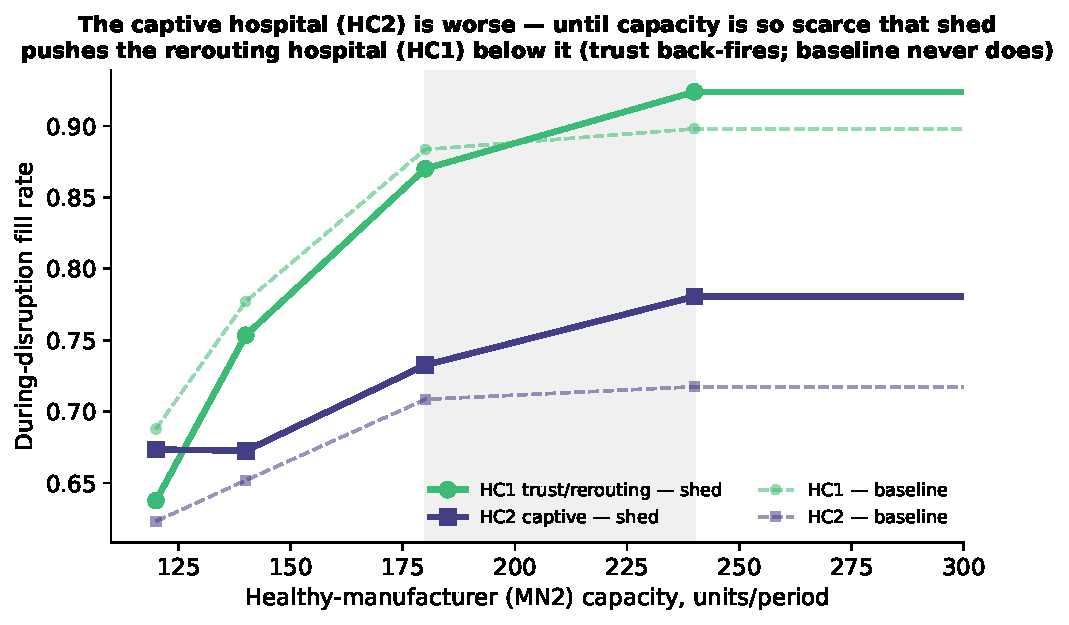
\includegraphics[width=0.82\textwidth]{figures/fig7_fill_by_capacity.pdf}
\caption{Per-hospital during-disruption fill vs.\ capacity (Table~1's fill columns). Under shed
(solid), the captive HC2 is worse than the rerouting HC1 at ample capacity, but as capacity
falls the lines \emph{cross} near MN2 = 125 --- the trust hospital, pushed fully onto the
congested healthy chain, ends up worse off. \emph{Why:} HC1's edge from concentrating on the
healthy chain shrinks as that chain starves, while the captive keeps harvesting the disrupted
chain's residual output ($\sim$18 units/period, which shed makes HC1 forfeit); below $\sim$125
the diversified captive overtakes the all-in trust hospital. The baseline reroute (dashed) never
inverts, so the back-firing is caused by the shed intervention --- echoing Doroudi et~al.\
(trust-based rerouting can leave the trust-sensitive buyer worse off), here via capacity
congestion rather than their Theory-of-Mind deprioritization.}
\label{fig:fillcap}
\end{figure}

\begin{figure}[h]\centering
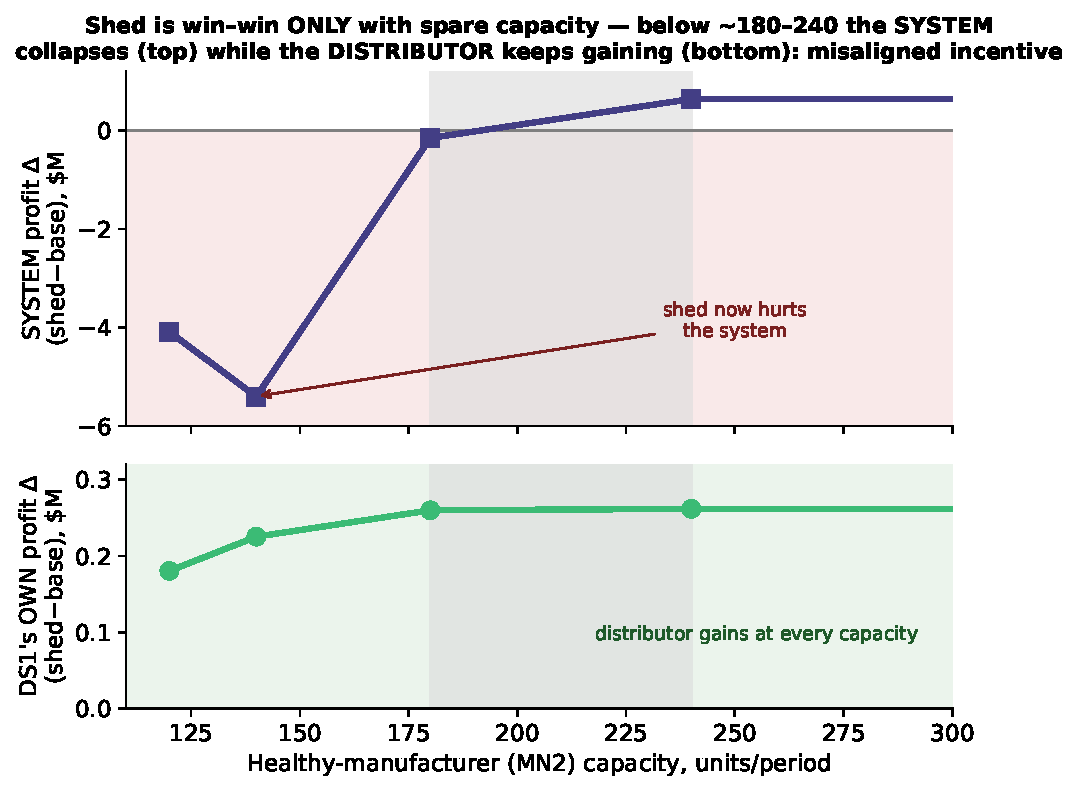
\includegraphics[width=0.82\textwidth]{figures/fig1_capacity_divergence.pdf}
\caption{Capacity sweep (Table~1), two panels with independent scales so both are readable: as
MN2 capacity falls, the \emph{system} (top) cliffs from $+0.6$M into $-5.4$M (red = shed hurts
the system), while DS1's \emph{own} profit (bottom, zoomed) stays positive at every capacity
($+0.26\to+0.18$M, green = always a gain). The gap between the panels \emph{is} the misaligned
incentive. (A single shared axis makes the DS1 line look flat against the system's swing.)}
\label{fig:div}
\end{figure}

\begin{figure}[h]\centering
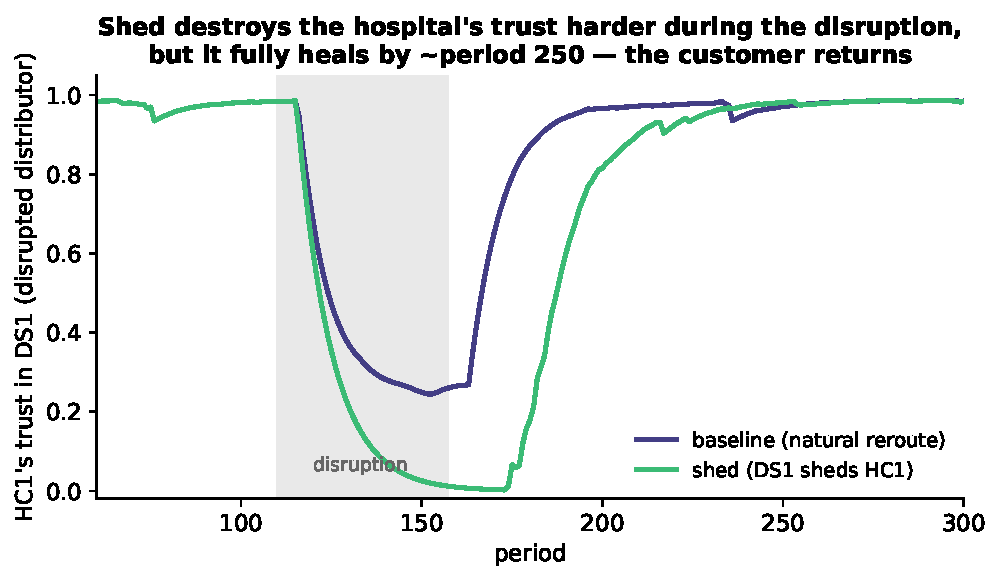
\includegraphics[width=0.80\textwidth]{figures/fig5_trust_trajectory.pdf}
\caption{The trust trajectory: HC1's trust in the disrupted distributor over the episode,
baseline vs shed. Shed drives trust to near zero during the disruption (sharper than the natural
reroute) but it fully recovers by $\sim$period~250 --- the customer is not lost.}
\label{fig:trust}
\end{figure}

\begin{figure}[h]\centering
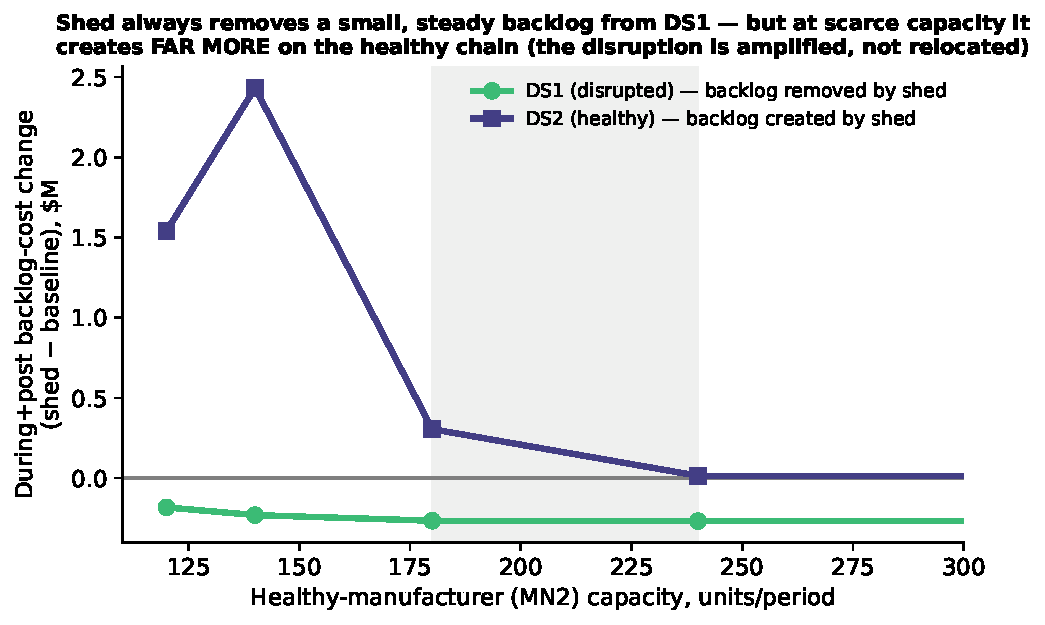
\includegraphics[width=0.72\textwidth]{figures/fig2_channel_during.pdf}
\caption{Where the backlog goes vs.\ capacity. Shed removes a small, steady backlog from DS1
($\sim-0.27$M at every capacity), but on the healthy chain DS2 it creates almost nothing at full
capacity ($+0.01$M) and \emph{far more} as capacity falls ($+2.4$M at MN2 = 140). So at scarce
capacity the disruption is \emph{amplified}, not relocated --- DS2 gains roughly ten times the
backlog DS1 sheds. (Table~\ref{tab:externality} is the per-agent snapshot at MN2 = 140.)}
\label{fig:chan}
\end{figure}

\begin{figure}[h]\centering
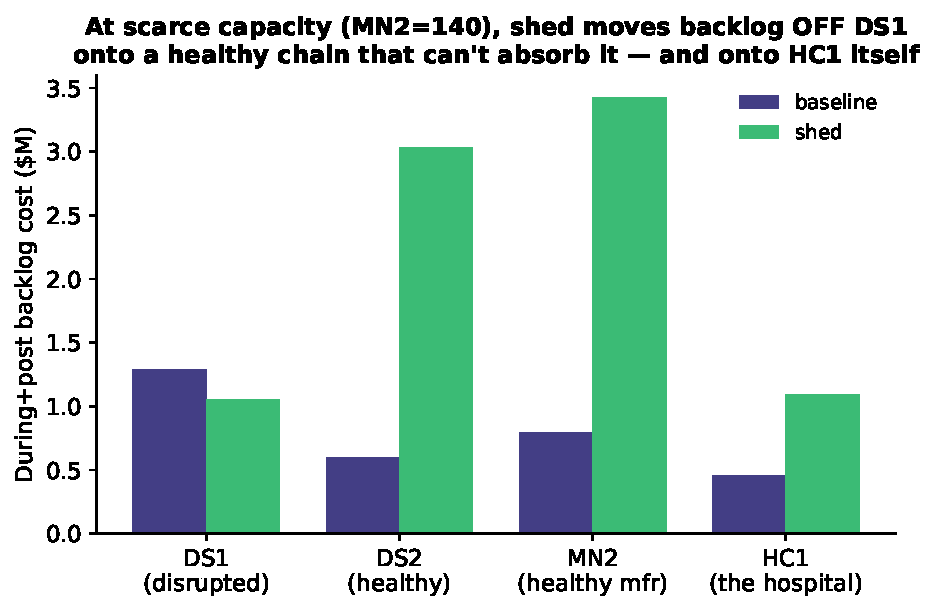
\includegraphics[width=0.78\textwidth]{figures/fig3_externality.pdf}
\caption{Table~\ref{tab:externality} as a plot: at scarce capacity (MN2 = 140) shed lowers DS1's
own backlog but explodes DS2's and MN2's, and HC1 itself ends up worse served --- the externality.}
\label{fig:ext}
\end{figure}

\begin{figure}[h]\centering
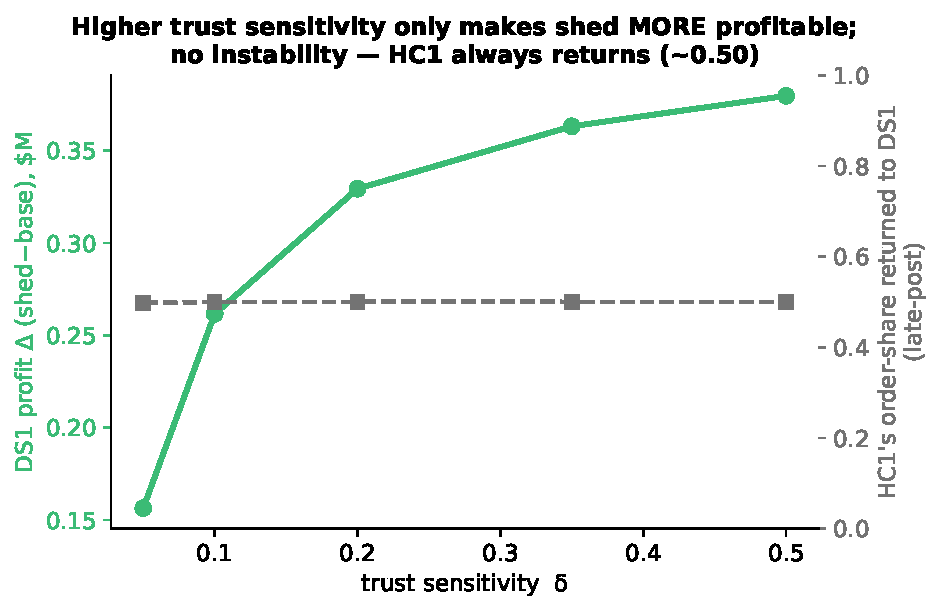
\includegraphics[width=0.78\textwidth]{figures/fig4_delta.pdf}
\caption{Table~4 as a plot: raising trust sensitivity $\delta$ only makes shed more profitable
for DS1; HC1's order-share always returns to $\sim$0.50 (right axis) --- no instability.}
\label{fig:delta}
\end{figure}

\begin{figure}[h]\centering
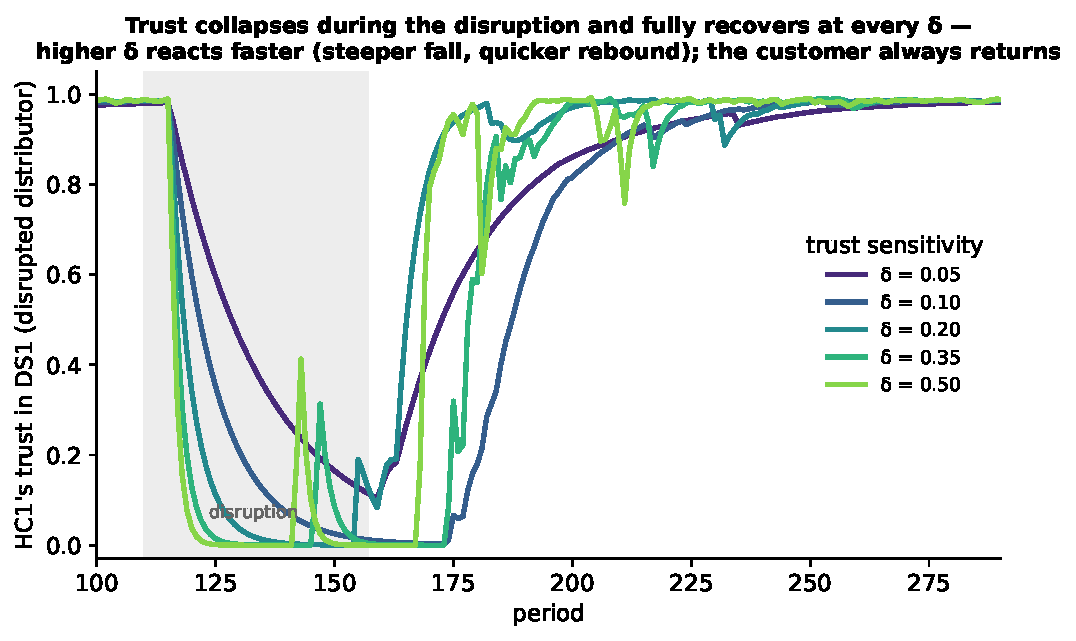
\includegraphics[width=0.84\textwidth]{figures/fig9_trust_by_delta.pdf}
\caption{HC1's trust in the disrupted distributor over the episode, one line per trust
sensitivity $\delta$ (shed policy) --- the same view as the baseline-vs-shed trust trajectory,
but across $\delta$. Trust collapses during the disruption (deeper and faster at higher $\delta$)
and fully recovers at every $\delta$: a single ramp down then back up, \emph{not} sustained
flip-flopping --- without Theory-of-Mind no agent strategically deprioritizes the customer, so
there is no switching loop. The brief high-$\delta$ spikes are reactive jitter (trust snapping to
individual deliveries). This one figure replaces the noisy oscillation-std and binary
``returns?'' summaries.}
\label{fig:trustdelta}
\end{figure}

\begin{figure}[h]\centering
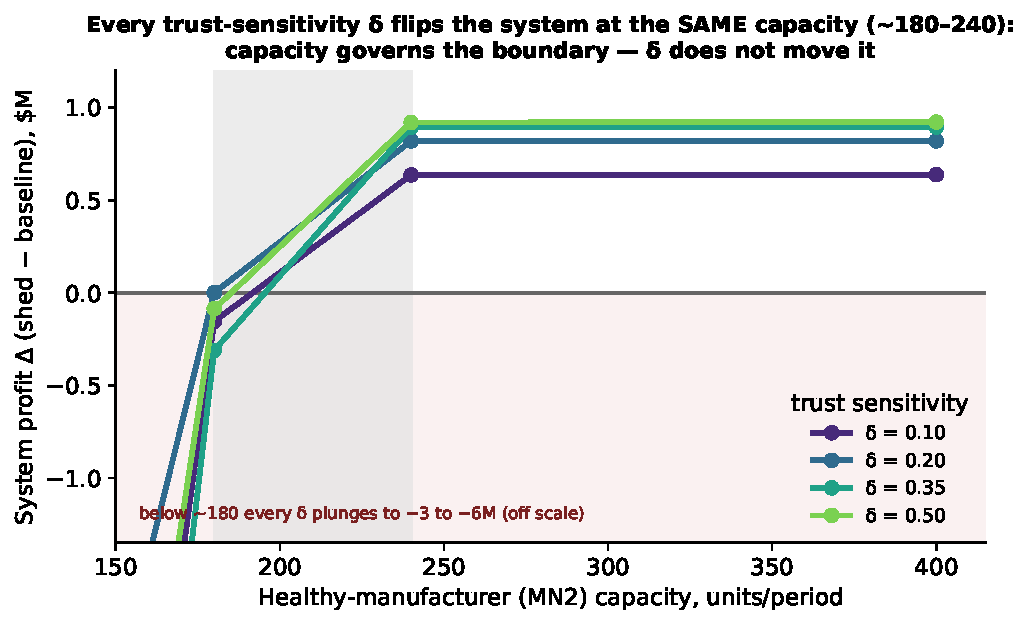
\includegraphics[width=0.82\textwidth]{figures/fig6_grid_heatmap.pdf}
\caption{System profit $\Delta$ vs.\ capacity, one line per trust sensitivity $\delta$ (the
$\delta\times$capacity grid, Table~\ref{tab:grid}). Every $\delta$ line crosses zero at the same
capacity ($\sim$180--240): \textbf{capacity governs the flip boundary}; $\delta$ only scales the
magnitude above it, never moving the boundary. (Below $\sim$180 all $\delta$ plunge to $-3$ to
$-6$M, off scale; HC1 returns to $\sim$0.50 in every cell, so there is no instability.)}
\label{fig:grid}
\end{figure}

\section{Robustness: two trust-based hospitals}

The thesis world has one trust + one captive hospital; making \emph{both} trust-based (rung-b,
existing data, slack regime) removes the captive anchor. Result: the two hospitals become
symmetric (during fill-dispersion HC1$-$HC2 falls $+0.181\to-0.000$) and DS1 is \emph{better off}
($-1{,}217{,}927\to-845{,}264$, i.e.\ $+372$k; during backlog cost $-193$k; same under urgent20,
$+403$k) --- with no captive to keep serving, it sheds backlog from both. So the captive-vs-trust
composition of the \emph{second} hospital is second-order for the disrupted distributor. (Two
follow-ups would each need a new run: shedding \emph{within} the two-trust world, and the
two-trust world under the capacity stress of \S1.)

\section{Shed's recovery dynamics}

Fig.~\ref{fig:chain} traces shed's effect on the disrupted distributor period by period (anchor,
full capacity). Shed lowers DS1's backlog during the disruption and trims its ordering --- but
its recovery inventory glut is \emph{larger}, not smaller (peak $\sim$227 vs 186; overshoot
$+159$ vs $+118$). The reason: shed reduces backlog by shedding the demand (HC1), and that demand
has not returned when supply recovers, so the distributor sits on inventory with little to serve.
So the intuitive chain ``less backlog $\to$ less ordering $\to$ smaller glut'' breaks at the last
link for shed --- it trades a smaller during-disruption backlog for a larger recovery glut. (The
extra glut is holding cost, cheap relative to the backlog penalty shed avoids, so DS1 still nets
the $+262$k gain of \S1; the glut is a real dynamic, not a reversal of the headline.)

\begin{figure}[h]\centering
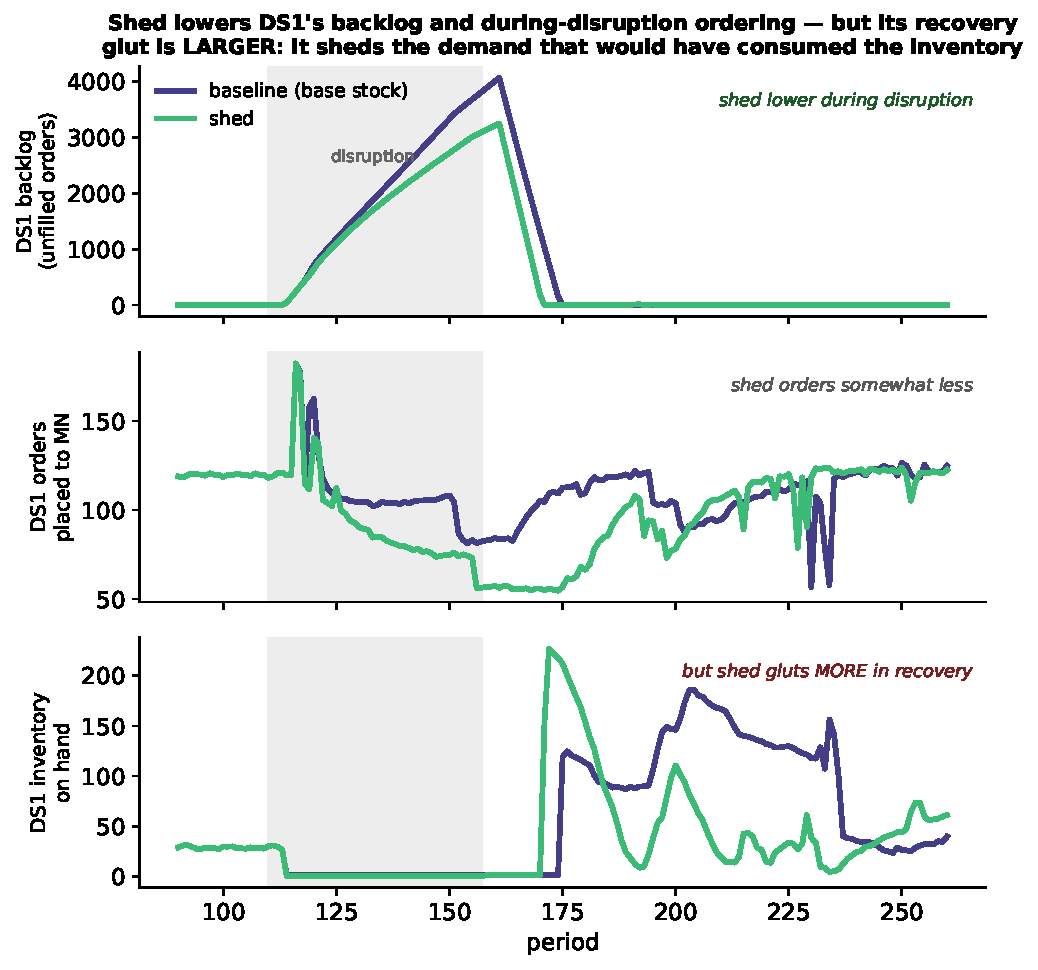
\includegraphics[width=0.74\textwidth]{figures/fig8_chain_reaction.pdf}
\caption{Recovery dynamics for DS1 (anchor): backlog (top), orders placed to the manufacturer
(middle), inventory on hand (bottom); baseline vs shed, with the disruption window shaded. Shed's
backlog and ordering are lower during the disruption, but its recovery inventory overshoot is
larger --- the shed demand (HC1) has not returned to consume the inventory.}
\label{fig:chain}
\end{figure}

\end{document}
